%----------------------------------------------------------------------------
\chapter{Software Architecture}\label{Ch2}
%----------------------------------------------------------------------------
Now that we have a basic understanding of the requirements, the architecture may be chosen. 

%----------------------------------------------------------------------------
\section{Serverless Architecture}
%----------------------------------------------------------------------------

As the vigilant reader probably noticed already, I will be developing a serverless application \cite{AzurePatterns}. I will rely on the things I already discussed in the Introduction  (Chapter~\ref{Introduction}). There are a few things to take into account.  This allows me not to care too much about where and how my application will be running. I don't have to configure a server or worry about whether or not I will have enough storage space locally.

There are multiple options to choose from if one would like to start working with serverless \cite{ServerlessPlatforms}. The most popular cloud computing platforms are Amazon Web Services \cite{AWS}, Google Cloud Platform \cite{GCP}, and Microsoft Azure \cite{MA}, each of which has it's own advantages and drawbacks. All of these provide some sort of FaaS (see Chapter \ref{Introduction}), in most cases this service is called Functions which can be used to run user functions which interact with other cloud components e.g.\ databases.

I will specifically work with Microsoft Azure in alignment with the thesis description.

%----------------------------------------------------------------------------
\section{Architecture Patterns Overview}
%----------------------------------------------------------------------------
 Although there seems to be a small misunderstanding about whether the serverless architecture stands in an either-or relation with the following patterns, in my understanding a serverless solution can be implemented along with the following patterns given that the pattern fits into the concept of serverless. Now I will look at some of the basic architecture styles. The goal is to find a pattern with which serverless can be used intuitively \cite{AzurePatterns}\cite{SoftArch}\cite{MarkRichards}.

\subsection{Monoliths}

Monolith applications have one big code base. This way the whole application can be deployed at once and has an unified infrastructure, although in a team it can be problematic to work together and decide who is responsible for which part of the code. As a one-person development team, I could have used this pattern. Conversely, I have some experience with this approach from previous courses and it is not entirely positive. Refactoring or minor changes in the code cause a lot of work on other parts of the app. This also means the whole thing has to be built and deployed again. If something goes wrong, debugging even a medium-sized application can be very challenging, because the problem could come from basically anywhere.

\subsection{Layered or N-Tier}

Layered applications divide the application logic into horizontal layers. Each of these has a specific role in the application and only neighbours communicate with each other. Commonly these include user interface, business logic and data access. This is an often used pattern and it has advantages. E.g.\ when changes occur in a layer, other layers can stay untouched or work with minimal modifications. On the contrary, according to \cite{Patterns}, the situation, where layers simply pass on data with little or no logic performed on it can occur often with this pattern. Also the implemented pattern tends to lean towards a layered monolith, which causes the same problems on a smaller scale.

\subsection{Microservices}

 Microservices architecture \cite{MicroservicesArch} incorporates multiple small sized services with different responsibilities in the application logic. The strength of this approach is that the services only loosely or not at all rely on each other if it is designed correctly. They can be implemented in their own, differing technology stacks, as each service has their own APIs and they communicate through these with each other and the exact implementation is hidden. This also means, that they can work on entirely different data stores and also each of them manages their own data and don't rely on external layers or services to do so. Contrary to monolithic or layered applications, microservices can be deployed one-by-one. Developers don't have to work with a boundlessly expanding code base which means a major vulnerability to bugs that may block the deployment of the entire application.
On the down side, if the microservices structure gets expanded, it can become challenging to follow how to reach each of the services. In case of a bad design, microservices can cause more inconvenience than benefit, leading to hardly maintainable data persistence and overly complicated infrastructure. If responsibility areas are partitioned inefficiently, it can lead to too much communication between the APIs, which will deteriorate the response time of the application.

To give an example of bad design, at one point during the development of this application I wanted to spare some coding by not separating a NoSQL document into different data stores. This resulted in a scenario, where two microservices managed different parts of the same document. Obviously this means, that each of them has to know about and contain the structure of this document which means these are redundantly written twice and also caused me some problem, where I forgot to modify both of them and it resulted in a lengthy debugging session as the document structure became inconsistent. The solution here would be either to split the database document into two or merge the two microservices into one service.

%----------------------------------------------------------------------------
\section{Restaurant Application Architecture}
%----------------------------------------------------------------------------

Reading about function apps they seemed pretty easy to create and maintain. For me it seems to be intuitive to create one function app for one small part of business logic. That's why I decided on a microservices architecture. I thought of something similar to this example \cite{FuncAppsCosmosDB}, which seemed more comprehensible than some of the architecture designs I've run into. \figref{AppArch}

\begin{figure}[!ht]
	\centering
	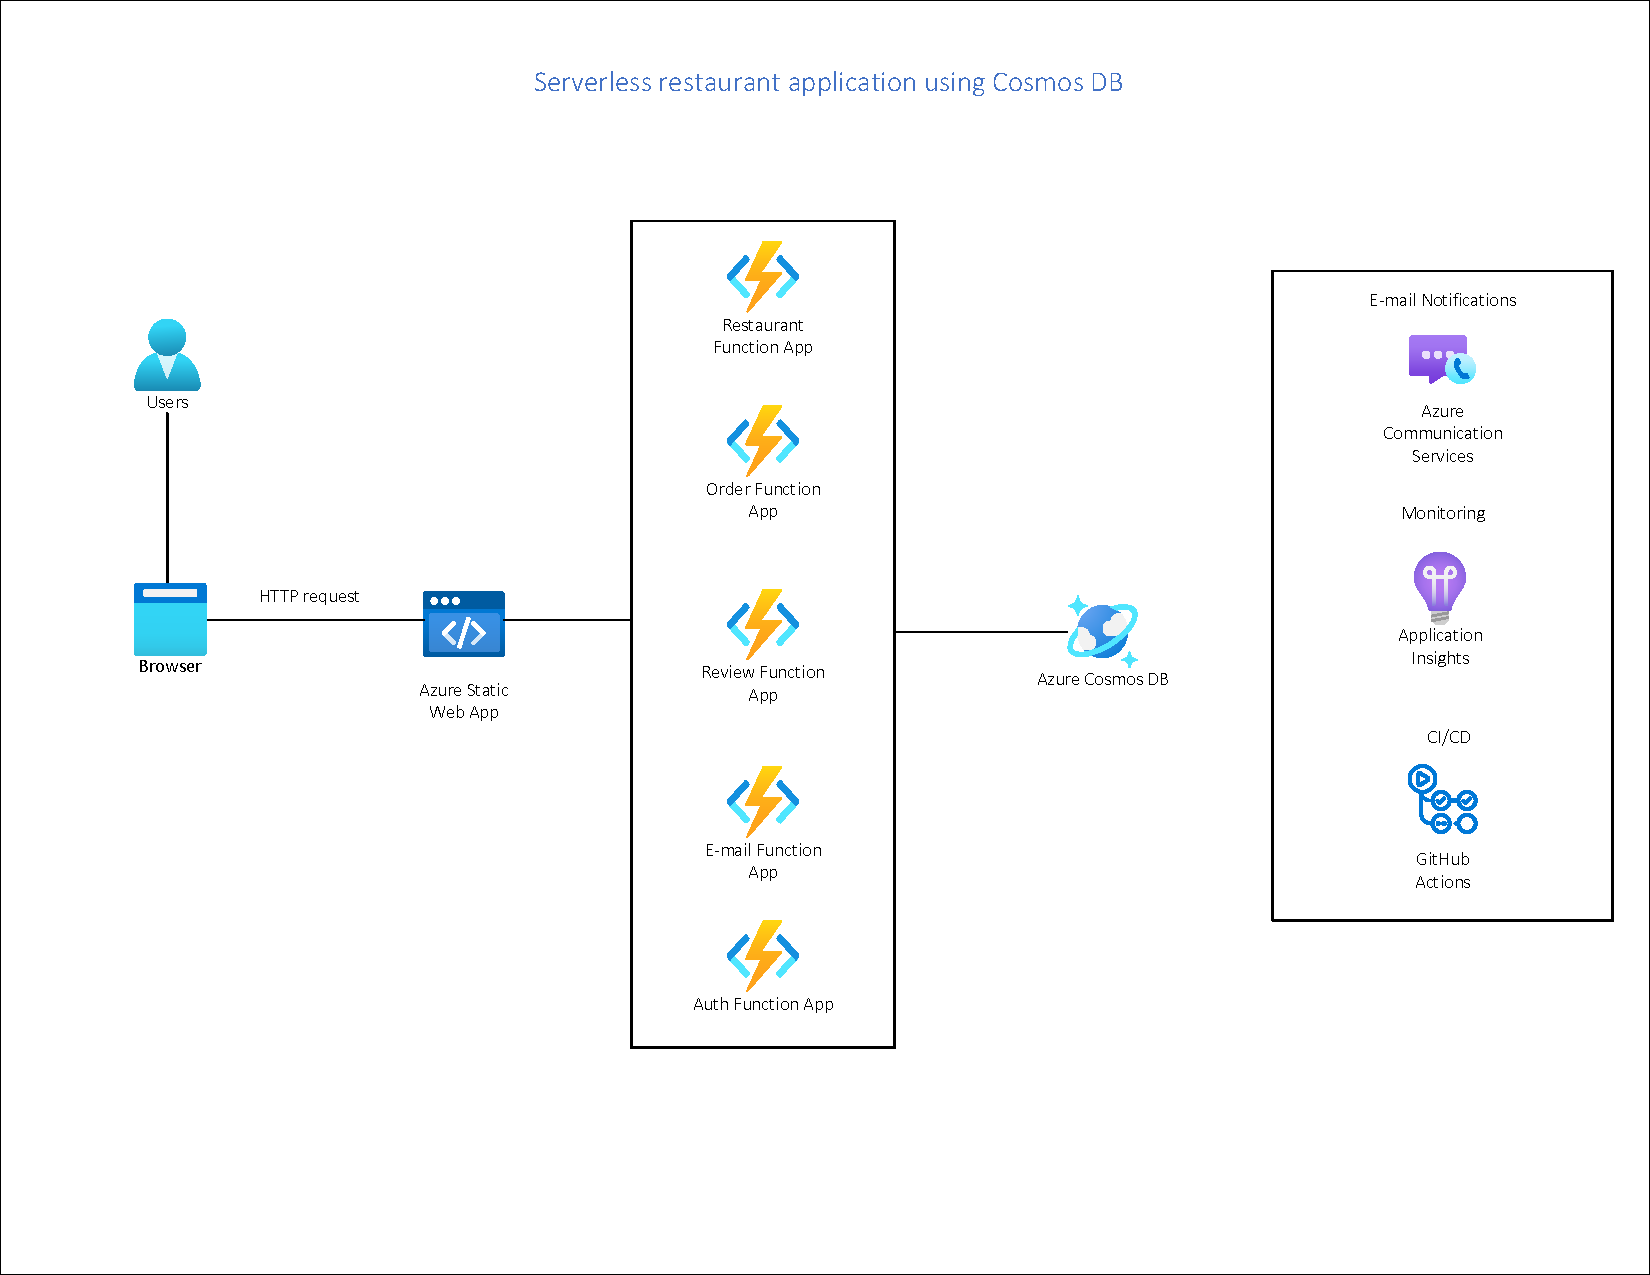
\includegraphics[width=150mm, keepaspectratio]{figures/AppArch}
	\caption{Restaurant application architecture diagram} 
	\label{fig:AppArch}
\end{figure}

%----------------------------------------------------------------------------
\subsection{Workflow}
%----------------------------------------------------------------------------

The architecture gets its input data from the user, who will send HTTP requests to an Azure Static Web App via the browser. The requests will trigger the underlying Function Apps and save or read the application data from Cosmos DB, which will be the architecture's main data service solution. I would like to use Azure Communication Services for e-mail notifications. Application Insights will provide debugging options on Azure. Finally, the app will be integrated with GitHub Actions to build and publish it to Azure.

%----------------------------------------------------------------------------
\subsection{Components}
%----------------------------------------------------------------------------

The components of my thought-out architecture are the following:

\begin{itemize}
	\item \textbf{Azure Static Web Apps} \emph{"is a service that automatically builds and deploys full stack web apps to Azure from a code repository."} It can interact with GitHub, so when a certain action is executed e.g.\ commit, the app builds and gets deployed automatically.\cite{StaticWebApps}
	
	\item \textbf{Azure Function Apps} is a FaaS platform to deploy compute-on-demand code without managing any underlying systems. \cite{ArchExample1}
	
	\item \textbf{Azure Cosmos DB} is a fully managed NoSQL database with nearly limitless scale. \cite{ArchExample1}
	
	\item \textbf{Azure Application Insights} is the native Application Perfirmance Management service in Azure which can be easily integrated with Web Apps and Azure Functions. \cite{ArchExample1}
	
	\item \textbf{Azure Communication Services} are cloud-based services which allow the developer to easily integrate different communication formats into his application such as e-mail, SMS or video. \cite{CommunicationServices}
	
	\item \textbf{GitHub Actions} According to GitHub, \emph{"GitHub Actions is a continuous integration and continuous delivery (CI/CD) platform that allows you to automate your build, test, and deployment pipeline. You can create workflows that build and test every pull request to your repository, or deploy merged pull requests to production."} \cite{GitHubActions}
	
\end{itemize}





